% Options for packages loaded elsewhere
\PassOptionsToPackage{unicode}{hyperref}
\PassOptionsToPackage{hyphens}{url}
%
\documentclass[
]{bxjsbook}
\usepackage{amsmath,amssymb}
\usepackage{lmodern}
\usepackage{iftex}
\ifPDFTeX
  \usepackage[T1]{fontenc}
  \usepackage[utf8]{inputenc}
  \usepackage{textcomp} % provide euro and other symbols
\else % if luatex or xetex
  \usepackage{unicode-math}
  \defaultfontfeatures{Scale=MatchLowercase}
  \defaultfontfeatures[\rmfamily]{Ligatures=TeX,Scale=1}
\fi
% Use upquote if available, for straight quotes in verbatim environments
\IfFileExists{upquote.sty}{\usepackage{upquote}}{}
\IfFileExists{microtype.sty}{% use microtype if available
  \usepackage[]{microtype}
  \UseMicrotypeSet[protrusion]{basicmath} % disable protrusion for tt fonts
}{}
\makeatletter
\@ifundefined{KOMAClassName}{% if non-KOMA class
  \IfFileExists{parskip.sty}{%
    \usepackage{parskip}
  }{% else
    \setlength{\parindent}{0pt}
    \setlength{\parskip}{6pt plus 2pt minus 1pt}}
}{% if KOMA class
  \KOMAoptions{parskip=half}}
\makeatother
\usepackage{xcolor}
\usepackage{color}
\usepackage{fancyvrb}
\newcommand{\VerbBar}{|}
\newcommand{\VERB}{\Verb[commandchars=\\\{\}]}
\DefineVerbatimEnvironment{Highlighting}{Verbatim}{commandchars=\\\{\}}
% Add ',fontsize=\small' for more characters per line
\usepackage{framed}
\definecolor{shadecolor}{RGB}{248,248,248}
\newenvironment{Shaded}{\begin{snugshade}}{\end{snugshade}}
\newcommand{\AlertTok}[1]{\textcolor[rgb]{0.94,0.16,0.16}{#1}}
\newcommand{\AnnotationTok}[1]{\textcolor[rgb]{0.56,0.35,0.01}{\textbf{\textit{#1}}}}
\newcommand{\AttributeTok}[1]{\textcolor[rgb]{0.77,0.63,0.00}{#1}}
\newcommand{\BaseNTok}[1]{\textcolor[rgb]{0.00,0.00,0.81}{#1}}
\newcommand{\BuiltInTok}[1]{#1}
\newcommand{\CharTok}[1]{\textcolor[rgb]{0.31,0.60,0.02}{#1}}
\newcommand{\CommentTok}[1]{\textcolor[rgb]{0.56,0.35,0.01}{\textit{#1}}}
\newcommand{\CommentVarTok}[1]{\textcolor[rgb]{0.56,0.35,0.01}{\textbf{\textit{#1}}}}
\newcommand{\ConstantTok}[1]{\textcolor[rgb]{0.00,0.00,0.00}{#1}}
\newcommand{\ControlFlowTok}[1]{\textcolor[rgb]{0.13,0.29,0.53}{\textbf{#1}}}
\newcommand{\DataTypeTok}[1]{\textcolor[rgb]{0.13,0.29,0.53}{#1}}
\newcommand{\DecValTok}[1]{\textcolor[rgb]{0.00,0.00,0.81}{#1}}
\newcommand{\DocumentationTok}[1]{\textcolor[rgb]{0.56,0.35,0.01}{\textbf{\textit{#1}}}}
\newcommand{\ErrorTok}[1]{\textcolor[rgb]{0.64,0.00,0.00}{\textbf{#1}}}
\newcommand{\ExtensionTok}[1]{#1}
\newcommand{\FloatTok}[1]{\textcolor[rgb]{0.00,0.00,0.81}{#1}}
\newcommand{\FunctionTok}[1]{\textcolor[rgb]{0.00,0.00,0.00}{#1}}
\newcommand{\ImportTok}[1]{#1}
\newcommand{\InformationTok}[1]{\textcolor[rgb]{0.56,0.35,0.01}{\textbf{\textit{#1}}}}
\newcommand{\KeywordTok}[1]{\textcolor[rgb]{0.13,0.29,0.53}{\textbf{#1}}}
\newcommand{\NormalTok}[1]{#1}
\newcommand{\OperatorTok}[1]{\textcolor[rgb]{0.81,0.36,0.00}{\textbf{#1}}}
\newcommand{\OtherTok}[1]{\textcolor[rgb]{0.56,0.35,0.01}{#1}}
\newcommand{\PreprocessorTok}[1]{\textcolor[rgb]{0.56,0.35,0.01}{\textit{#1}}}
\newcommand{\RegionMarkerTok}[1]{#1}
\newcommand{\SpecialCharTok}[1]{\textcolor[rgb]{0.00,0.00,0.00}{#1}}
\newcommand{\SpecialStringTok}[1]{\textcolor[rgb]{0.31,0.60,0.02}{#1}}
\newcommand{\StringTok}[1]{\textcolor[rgb]{0.31,0.60,0.02}{#1}}
\newcommand{\VariableTok}[1]{\textcolor[rgb]{0.00,0.00,0.00}{#1}}
\newcommand{\VerbatimStringTok}[1]{\textcolor[rgb]{0.31,0.60,0.02}{#1}}
\newcommand{\WarningTok}[1]{\textcolor[rgb]{0.56,0.35,0.01}{\textbf{\textit{#1}}}}
\usepackage{longtable,booktabs,array}
\usepackage{calc} % for calculating minipage widths
% Correct order of tables after \paragraph or \subparagraph
\usepackage{etoolbox}
\makeatletter
\patchcmd\longtable{\par}{\if@noskipsec\mbox{}\fi\par}{}{}
\makeatother
% Allow footnotes in longtable head/foot
\IfFileExists{footnotehyper.sty}{\usepackage{footnotehyper}}{\usepackage{footnote}}
\makesavenoteenv{longtable}
\usepackage{graphicx}
\makeatletter
\def\maxwidth{\ifdim\Gin@nat@width>\linewidth\linewidth\else\Gin@nat@width\fi}
\def\maxheight{\ifdim\Gin@nat@height>\textheight\textheight\else\Gin@nat@height\fi}
\makeatother
% Scale images if necessary, so that they will not overflow the page
% margins by default, and it is still possible to overwrite the defaults
% using explicit options in \includegraphics[width, height, ...]{}
\setkeys{Gin}{width=\maxwidth,height=\maxheight,keepaspectratio}
% Set default figure placement to htbp
\makeatletter
\def\fps@figure{htbp}
\makeatother
\setlength{\emergencystretch}{3em} % prevent overfull lines
\providecommand{\tightlist}{%
  \setlength{\itemsep}{0pt}\setlength{\parskip}{0pt}}
\setcounter{secnumdepth}{5}
\usepackage{booktabs}
\usepackage{ctex}

\renewcommand{\contentsname}{目次}

%\usepackage{xeCJK}
%\usepackage{CJKutf8} 
%\usepackage{zxjatype}
%\usepackage{xltxtra} 
%\usepackage{fontspec}
%\setCJKmainfont{Noto Serif CJK TC}
%\setCJKsansfont{Noto Sans CJK TC}
%\setCJKmonofont{Noto Sans Mono CJK TC}
%\setCJKmainfont{IPAMincho}
%\setCJKsansfont{IPAGothic}
%\setCJKmonofont{IPAGothic}
%\RequirePackage{plautopatch}
\ifLuaTeX
  \usepackage{selnolig}  % disable illegal ligatures
\fi
\usepackage[]{natbib}
\bibliographystyle{apalike}
\IfFileExists{bookmark.sty}{\usepackage{bookmark}}{\usepackage{hyperref}}
\IfFileExists{xurl.sty}{\usepackage{xurl}}{} % add URL line breaks if available
\urlstyle{same} % disable monospaced font for URLs
\hypersetup{
  pdftitle={データサイエンスをはじめましょう - Data Science for All -},
  pdfauthor={John Doe},
  hidelinks,
  pdfcreator={LaTeX via pandoc}}

\title{データサイエンスをはじめましょう - Data Science for All -}
\author{John Doe}
\date{2023-02-17}

\usepackage{amsthm}
\newtheorem{theorem}{Theorem}[section]
\newtheorem{lemma}{Lemma}[section]
\newtheorem{corollary}{Corollary}[section]
\newtheorem{proposition}{Proposition}[section]
\newtheorem{conjecture}{Conjecture}[section]
\theoremstyle{definition}
\newtheorem{definition}{Definition}[section]
\theoremstyle{definition}
\newtheorem{example}{Example}[section]
\theoremstyle{definition}
\newtheorem{exercise}{Exercise}[section]
\theoremstyle{definition}
\newtheorem{hypothesis}{Hypothesis}[section]
\theoremstyle{remark}
\newtheorem*{remark}{Remark}
\newtheorem*{solution}{Solution}
\begin{document}
\maketitle

{
\setcounter{tocdepth}{2}
\tableofcontents
}
\hypertarget{about}{%
\section{この文書について}\label{about}}

データサイエンスを始めてみませんか。

データサイエンスは、広い意味をもったことばで、一口に、まなび始めると言っても、さまざまな始め方があると思います。本書では、そのひとつを提案するとともに、共に学んでいきたいと願って、書き始めました。

みなさんも一緒にデータサイエンスを学んでみませんか。

\hypertarget{ux8457ux8005ux306bux3064ux3044ux3066}{%
\subsection{著者について}\label{ux8457ux8005ux306bux3064ux3044ux3066}}

著者は、大学の学生の時以来、数学を学び、大学で教え、2019年春に退職。それ以来、少しずつ、データサイエンスを学んでいます。

幸運にも、2019年9月の日本数学会教育委員会主催教育シンポジウムで、「文理共通して行う数理・データサイエンス教育」という題で、話す機会が与えられ、その後、あることが契機となり、2020年度から、毎年、冬に、大学院一般向け(分野の指定なし)の授業、「研究者のためのデータ分析(Data Analysis for Researchers)」を担当しています。複数の教員で担当しますが、基本的な部分は、わたしが教えています。受講生は20人程度ですが、殆どが、外国人。それも、多国籍で、多くても一国から三人程度。英語で教えています。

\hypertarget{ux30b3ux30f3ux30d4ux30e5ux30fcux30bfux8a00ux8a9eux306bux3064ux3044ux3066}{%
\subsection{コンピュータ言語について}\label{ux30b3ux30f3ux30d4ux30e5ux30fcux30bfux8a00ux8a9eux306bux3064ux3044ux3066}}

統計解析のために開発された R を使います。いずれは、python についても触れたいと思いますが、プログラミングの経験がない方も含めて、最初にデータサイエンスを学ぶには、R は最適だと考えています。特に、R Studio IDE(integrated development environment, 統合開発環境) で、R を使うことがとても、簡単になっています。さらに、簡単なものであれば、Posit Cloud で試したり、共有することも可能です。また、再現性(Reproducibility)や、なにを実行しているのかの説明を同時に記述すること(Literate Programming)は、非常に重要ですが、その記述も、R Markdown によって、可能いなっています。この文書も、R Markdown の一つの形式の、bookdown を利用しています。最後に、Bookdown に関連して、膨大な数の、参考書も、無償で提供されており、オンラインで読むことができることも、R をお薦めする理由です。

ただし、日本語のものは、まだ十分とは言えない状況です。この文書を書き始めたのも、すこしでも、お役に立つことができればとの、気持ちが背景にあります。

\hypertarget{ux8a00ux8a9eux306bux3064ux3044ux3066}{%
\subsection{言語について}\label{ux8a00ux8a9eux306bux3064ux3044ux3066}}

ご覧の通り、本書は、日本語で書かれています。用語は、英語、あるいは、英語を追記、または、英語をカタカナにしただけのものを使用する可能性が大きいですが、説明は、極力、日本語で書いていく予定です。

しかし、基本的に、コード(プログラムの記述)には、日本語を使わないで書いていく予定です。とくに、初心者にとっては、日本語の扱いは、負担になることが多いからです。最近は、コードの中で日本語を使用しても、ほとんど、問題は起きないように思います。そうであっても、世界の人の共通言語として、プログラム言語を学んでいくときには、日本語を使わないことは意義があると思います。

少し慣れてきて、日本語のデータなどを扱うときには、コードにも日本語を使う必要ができていますから、日本語の利用についても、追って説明していきます。

最初は、みなさんも、変数(variable)や、オブジェクト(object)に名前をつけるときは、半角英数を使い、日本語は、使わないようにすることをお勧めします。

\hypertarget{introduction}{%
\section{はじめに}\label{introduction}}

\begin{quote}
Data Science: データ (Data) を活用して課題を発見・探求し、適切な解決策を探る意思決定のための科学(Decision Science)で、 エンピリカル(Empirical Study)すなわち、理論ではなく、実証性を特徴とする。 データから得られる特徴を表示するとともに、数理モデルを適用し・機械学習などで評価し・アルゴリズムを策定する数理的思考を通して得られた結果を、可視化などによってコミュニケーションをおこない、共有し、他者の意見を聞き理解する努力をしながら、さらに課題について、あらたにデータを活用して考え、検証し、適切な解決策がもたらす新たな課題も予測しながら、調整をはかる。
\end{quote}

\hypertarget{part-part-i-public-data}{%
\part{PART I PUBLIC DATA}\label{part-part-i-public-data}}

\hypertarget{publicdata}{%
\section{Public Data}\label{publicdata}}

まずは、パブリックデータを見てみましょう。大きな機関のパグリックデータには、ダッシュボード(dashboard)と呼ばれている、パラメタを変更して、そのグラフを描くなどの機能が付いているものもあります。

\hypertarget{world-bank}{%
\subsection{World Bank}\label{world-bank}}

\hypertarget{open-government-data-toolkit-open-data-defined}{%
\subsubsection{\texorpdfstring{\href{http://opendatatoolkit.worldbank.org}{Open Government Data Toolkit}: \href{http://opendatatoolkit.worldbank.org/en/essentials.html}{Open Data Defined}}{Open Government Data Toolkit: Open Data Defined}}\label{open-government-data-toolkit-open-data-defined}}

The term \textbf{Open Data} has a very precise meaning. Data or content is open if anyone is free to use, re-use or redistribute it, subject at most to measures that preserve provenance and openness.

\begin{enumerate}
\def\labelenumi{\arabic{enumi}.}
\tightlist
\item
  The data must be \emph{legally open}, which means they must be placed in the public domain or under liberal terms of use with minimal restrictions.
\item
  The data must be \emph{technically open}, which means they must be published in electronic formats that are machine readable and non-proprietary, so that anyone can access and use the data using common, freely available software tools. Data must also be publicly available and accessible on a public server, without password or firewall restrictions. To make Open Data easier to find, most organizations create and manage Open Data catalogs.
\end{enumerate}

\hypertarget{worldbank-data}{%
\subsection{Worldbank Data}\label{worldbank-data}}

\begin{itemize}
\tightlist
\item
  Climate Change Knowledge Portal: \url{https://climateknowledgeportal.worldbank.org}

  \begin{itemize}
  \tightlist
  \item
    country summary
  \end{itemize}
\end{itemize}

\hypertarget{world-bank-wdi---world-development-indicaters}{%
\subsection{World Bank: WDI - World Development Indicaters}\label{world-bank-wdi---world-development-indicaters}}

\begin{itemize}
\tightlist
\item
  World Bank: \url{https://www.worldbank.org}
\item
  \href{https://www.worldbank.org/en/who-we-are}{Who we are}:

  \begin{itemize}
  \tightlist
  \item
    To end extreme poverty: By reducing the share of the global population that lives in extreme poverty to 3 percent by 2030.
  \item
    To promote shared prosperity: By increasing the incomes of the poorest 40 percent of people in every country.
  \end{itemize}
\item
  World Bank Open Data: \url{https://data.worldbank.org}

  \begin{itemize}
  \tightlist
  \item
    Data Bank, World Development Indicators, etc.
  \end{itemize}
\end{itemize}

\hypertarget{world-development-indicator}{%
\subsubsection{World Development Indicator}\label{world-development-indicator}}

\begin{itemize}
\tightlist
\item
  \href{https://datatopics.worldbank.org/world-development-indicators/}{World Development Indicators (WDI)} : the World Bank's premier compilation of cross-country comparable data on development; 1400 time series indicators

  \begin{itemize}
  \tightlist
  \item
    Themes: Poverty and Inequality, People, Environment, Economy, States and Markets, Global Links
  \item
    Open Data \& DataBank: Explore data, Query database
  \item
    Bulk Download: Excel, CSV
  \item
    API Documentation
  \end{itemize}
\end{itemize}

\hypertarget{oecd}{%
\subsection{OECD}\label{oecd}}

OECD Data: \url{https://data.oecd.org/}

\hypertarget{un-data}{%
\subsection{UN Data}\label{un-data}}

UNdata: \url{https://data.un.org}

\hypertarget{our-world-in-data}{%
\subsection{Our World in Data}\label{our-world-in-data}}

owid: \url{https://ourworldindata.org/}

\hypertarget{eurostat}{%
\subsection{Eurostat}\label{eurostat}}

eurostat: \url{https://ec.europa.eu/eurostat}

\hypertarget{part-part-ii-basics}{%
\part{PART II BASICS}\label{part-part-ii-basics}}

\hypertarget{ronrstudio}{%
\section{R on R Studio}\label{ronrstudio}}

\hypertarget{ux306fux3058ux3081ux306b}{%
\subsection{はじめに}\label{ux306fux3058ux3081ux306b}}

R Studio で R を使うことを始めましょう。

このページの一番下に、簡単な解説ビデオがついています。

\hypertarget{r-ux3068-r-studio}{%
\subsection{R と R Studio}\label{r-ux3068-r-studio}}

\begin{quote}
R is a free software environment for statistical computing and graphics. It compiles and runs on a wide variety of UNIX platforms, Windows and MacOS. \url{https://www.r-project.org}
\end{quote}

\begin{quote}
R は、無償で提供されている、統計解析とグラフを描写する環境です。Windows、MacOS や、Linux で利用することが可能です。
\end{quote}

\begin{quote}
RStudio is an integrated development environment (IDE) for R and Python. It includes a console, syntax-highlighting editor that supports direct code execution, and tools for plotting, history, debugging, and workspace management. RStudio is available in open source and commercial editions and runs on the desktop (Windows, Mac, and Linux). \url{https://posit.co/products/open-source/rstudio/}
\end{quote}

\begin{quote}
RStudio は、R と Python のための、総合開発環境です。RStudio には、プログラムを実行したり、制御やジョブ管理のための、コンソール(console)、コードを書いたり、実行したりする、文書の編集をする、エディター(Editor)とともに、グラフを表示したり、履歴や、プログラムを修正するなどのための、さまざまなツールが付属しています。RStudio はオープンソースで提供され、Windows、Mac および、Linux で利用可能で、有償版のサービスと無償版を提供しています。
\end{quote}

R は、統計解析のためのシステムで、R Studio は、R(および Python)を利用するための、総合開発環境です。そこで、「R Studio で R を利用する」という表現をします。

\hypertarget{r-ux3068-r-studio-ux306eux30a4ux30f3ux30b9ux30c8ux30fcux30eb}{%
\subsection{R と R Studio のインストール}\label{r-ux3068-r-studio-ux306eux30a4ux30f3ux30b9ux30c8ux30fcux30eb}}

R と R Studio をインストールします。

両方とも、インストールすることが必要です。

\hypertarget{r-ux306eux30a4ux30f3ux30b9ux30c8ux30fcux30eb}{%
\subsubsection{R のインストール}\label{r-ux306eux30a4ux30f3ux30b9ux30c8ux30fcux30eb}}

\url{https://cloud.r-project.org}

上のリンクから、Windows、macOS または、Linux を選択して、インストールしてください。

macOS の場合は、M1, M2 など、最近の Apple Silicon の CPU で動くコンピュータか、以前の、Intel の CPU で動くものか、選択してください。Mac の左上の、りんごマークの、このコンピュータについてから、確認できます。

不明の場合は、「R のインストール」と検索してみてください。

\hypertarget{r-studio-ux306e-ux30a4ux30f3ux30b9ux30c8ux30fcux30eb}{%
\subsubsection{R Studio の インストール}\label{r-studio-ux306e-ux30a4ux30f3ux30b9ux30c8ux30fcux30eb}}

\url{http://www.rstudio.com/download}

上のリンクから、Windows 10/11 または、macOS 11+ を 選択してください。これら以外の、古いシステムのコンピュータの場合は、 下のサイトから、探してください。

\url{https://docs.posit.co/previous-versions/}

不明の場合は、「RStudio のインストール」と検索してみてください。

\hypertarget{ux30d7ux30edux30b8ux30a7ux30afux30c8---project}{%
\subsection{プロジェクト - Project}\label{ux30d7ux30edux30b8ux30a7ux30afux30c8---project}}

RStudio で R を利用する場合には、プロジェクトを作成することを強く勧めます。

\begin{enumerate}
\def\labelenumi{\arabic{enumi}.}
\item
  まず、R Studio を起動します。
\item
  上のメニューの、File から、New Project を選択します。New Directory(新しいディレクトリー)を選択し、プロジェクトを作成する Directory を決めて、名前をつけます。その名前が、プロジェクト名になります。
\end{enumerate}

\begin{itemize}
\tightlist
\item
  Directory(フォルダー)を指定してその名前をつけて、プロジェクトを作成します。
\item
  Directory が階層に分かれているときは、どこに作成するかを選択してから、名前をつけて、作成します。
\end{itemize}

\begin{enumerate}
\def\labelenumi{\arabic{enumi}.}
\setcounter{enumi}{2}
\item
  一旦、R Studio を終了してみましょう。
\item
  プロジェクトの起動には、いくつかの方法があります。
\end{enumerate}

\begin{itemize}
\tightlist
\item
  まず、R Studio を起動。一つしかプロジェクトがない場合は、そのプロジェクトが起動すると思います、。上に、プロジェクト名が掲載されていれば、問題ありません。
\item
  File から、Open Project を選択し、起動したい、プロジェクトの Directory(フォルダー)を選択して起動します。
\item
  File から、Recent Project(最近使ったプロジェクト)を選択すると、プロジェクト名が表示されますから、選択すると起動することができます。
\item
  コンピュータのプロジェクト入っているディレクトリー(フォルダー)をさがし、そこに、プロジェクト名.Rproj とあるものを見つけて、それを開くと、そのプロジェクトが起動します。
\end{itemize}

\begin{enumerate}
\def\labelenumi{\arabic{enumi}.}
\setcounter{enumi}{4}
\tightlist
\item
  作業後は、保存しますかと聞かれますから、保存して終了してください。
\end{enumerate}

\hypertarget{ux30b3ux30f3ux30bdux30fcux30ebux3067ux5b9fux884c---run-in-console}{%
\subsection{コンソールで実行 - Run in Console}\label{ux30b3ux30f3ux30bdux30fcux30ebux3067ux5b9fux884c---run-in-console}}

プログラム(コード)の実行は、いくつかの方法がありますが、一番、基本的な、コンソール(Console)での実行にすいて、説明します。Console は、R Studio の左下にあります。(左の枠が一つになっているかもしれません。その一番左のタブが Console です。選択されていない場合は、Console を選択してください。)

\hypertarget{ux6700ux521dux306eux56dbux3064}{%
\subsubsection{最初の四つ}\label{ux6700ux521dux306eux56dbux3064}}

下の、四つを、一つずつ、一番下の、\textgreater{} マークの次に書き(または、コピー・ペーストして)Return または、Enter キーを押してください。実行結果が、その下に出ます。最後の、\texttt{plot(cars)} は、\texttt{cars} というデータの、散布図が右下の、Plots タブに表示されます。

\begin{itemize}
\tightlist
\item
  \texttt{head(cars)}
\item
  \texttt{str(cars)}
\item
  \texttt{summary(cars)}
\item
  \texttt{plot(cars)}
\end{itemize}

エラーが表示されたら、もう一度、スペルを確認して、入力してみてください。

次のような、結果が表示されると思います。簡単な説明をつけます。

\begin{Shaded}
\begin{Highlighting}[]
\FunctionTok{head}\NormalTok{(cars)}
\CommentTok{\#\textgreater{}   speed dist}
\CommentTok{\#\textgreater{} 1     4    2}
\CommentTok{\#\textgreater{} 2     4   10}
\CommentTok{\#\textgreater{} 3     7    4}
\CommentTok{\#\textgreater{} 4     7   22}
\CommentTok{\#\textgreater{} 5     8   16}
\CommentTok{\#\textgreater{} 6     9   10}
\end{Highlighting}
\end{Shaded}

\texttt{head(cars)} は、\texttt{cars} という、R に付属している、データの、最初(頭 head)の6行を、表示します。

\begin{Shaded}
\begin{Highlighting}[]
\FunctionTok{str}\NormalTok{(cars)}
\CommentTok{\#\textgreater{} \textquotesingle{}data.frame\textquotesingle{}:    50 obs. of  2 variables:}
\CommentTok{\#\textgreater{}  $ speed: num  4 4 7 7 8 9 10 10 10 11 ...}
\CommentTok{\#\textgreater{}  $ dist : num  2 10 4 22 16 10 18 26 34 17 ...}
\end{Highlighting}
\end{Shaded}

\texttt{str(cars)} は、\texttt{cars} という、R に付属している、データの構造(structure)を表示します。\texttt{data.frame} とありますが、これは、矩形になったデータ(各列の長さがおなじ)の一番簡単なクラスの名前で、2変数、それぞれが、50 個の数値データ(numerical data) からなっていることがわかります。

head(cars)\texttt{では、縦に表示されていたものが、横に表示されています。}\(speed`、`\)dist\texttt{とありますが、}cars\(speed`, `cars\)dist\texttt{は、}cars` データの、それぞれの列を意味します。

\begin{Shaded}
\begin{Highlighting}[]
\FunctionTok{summary}\NormalTok{(cars)}
\CommentTok{\#\textgreater{}      speed           dist       }
\CommentTok{\#\textgreater{}  Min.   : 4.0   Min.   :  2.00  }
\CommentTok{\#\textgreater{}  1st Qu.:12.0   1st Qu.: 26.00  }
\CommentTok{\#\textgreater{}  Median :15.0   Median : 36.00  }
\CommentTok{\#\textgreater{}  Mean   :15.4   Mean   : 42.98  }
\CommentTok{\#\textgreater{}  3rd Qu.:19.0   3rd Qu.: 56.00  }
\CommentTok{\#\textgreater{}  Max.   :25.0   Max.   :120.00}
\end{Highlighting}
\end{Shaded}

\texttt{cars} データの概要(summary)が表示されます。各列(変数)について、最小値(Minimum)、小さい方から、4分の1を切り捨てたときの最小の値(1st Quadrant)、中央値(Median)、平均(Mean)、大きい方から、4分の1を切り捨てたときの最大の値(3rd Quadrant)、最大値(Maximum)が表示されます。

\begin{Shaded}
\begin{Highlighting}[]
\FunctionTok{plot}\NormalTok{(cars)}
\end{Highlighting}
\end{Shaded}

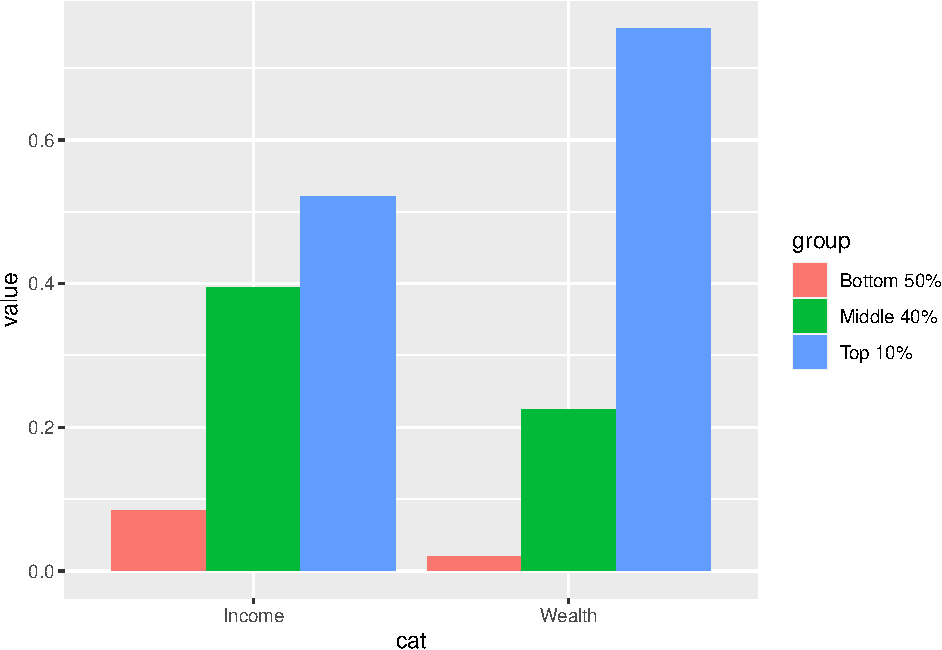
\includegraphics{21-r-on-rstudio_files/figure-latex/unnamed-chunk-5-1.pdf}

\hypertarget{ux30a2ux30b5ux30a4ux30f3ux30e1ux30f3ux30c8ux30d8ux30ebux30d7}{%
\subsubsection{アサインメント、ヘルプ}\label{ux30a2ux30b5ux30a4ux30f3ux30e1ux30f3ux30c8ux30d8ux30ebux30d7}}

コンソールで次のそれぞれを、試してみてください。

\begin{itemize}
\tightlist
\item
  \texttt{df\ \textless{}-\ cars}
\end{itemize}

\texttt{df} に、\texttt{cars} をアサインします。すなわち、\texttt{df} が、\texttt{cars} の内容に置き換わります。\texttt{cars} はデータですが、データを含む、オブジェクトの名前を設定するためにも使います。オブジェクト名は。英文字から始まれば、かなりの自由度がありますが、わたしは、英文字と数字と \texttt{\_}(underscore) 程度しか使わないようにしています。

\begin{itemize}
\tightlist
\item
  \texttt{head(df)}
\end{itemize}

\texttt{head(df)} は、\texttt{head(cars)} と同じ出力が得られます。

\begin{itemize}
\tightlist
\item
  \texttt{View(cars)}
\end{itemize}

左上の、窓枠が開き、\texttt{cars} の内容が表示されます。列名のところには、三角形も表示され、それを用いると、大きい順、小さい順などに、並び替えることも可能です。

\begin{itemize}
\tightlist
\item
  \texttt{?cars}
\end{itemize}

右下の、窓枠の Help タブに、\texttt{cars} の情報が表示されます。Help タブにある、虫眼鏡がついた、検索窓(search window)に、\texttt{cars} といれても、同じ結果が得られます。
内容を確認してください。

一番上には \texttt{cars\ \{datasets\}} とありますが、これは、\texttt{datasets} というパッケージの、\texttt{cars} だという意味です。そこで、\texttt{datasets} を調べてみましょう。

\begin{itemize}
\tightlist
\item
  \texttt{?datasets}
\end{itemize}

``The R Datasets Package'' だと書かれていて、さらに、

This package contains a variety of datasets. For a complete list, use library(help = ``datasets'').

さまざまなデータが含まれています。全てのリストをみるには、\texttt{library(help\ =\ "datasets")} を使ってください。

とありますから、\texttt{library(help\ =\ "datasets")} をコンソールに入力してみてください。

\begin{itemize}
\tightlist
\item
  \texttt{library(help\ =\ "datasets")}
\end{itemize}

左上の窓枠に、リストが表示されます。古いデータばかりですが、例として使うには、十分すぎるぐらいの、数のデータがあります。これらは、Toy Data(おもちゃのデータ)と呼ばれることもあります。

\texttt{cars} も見つかりましたか。

\hypertarget{ux304aux3059ux3059ux3081}{%
\subsubsection{おすすめ}\label{ux304aux3059ux3059ux3081}}

コンピュータのシステムが、日本語であると、R の言語も日本語になっているはずです。そこで、エラーが発生すると、一部、日本語で表示されます。しかし、ネット上などで、そのエラーの対応を検索するときは、英語のエラーメッセージで検索した方が、解決方法が得られる可能性が高いので、わたしは、英語に設定しています。英語にするには、Console で次のようにします。

言語を英語に設定:\texttt{Sys.setenv(LANG\ =\ "en")}

RStudio を終了して、もう一度起動すると、日本語に戻っていると思います。ですから、作業の最初、または、エラーが出たら、変更することをお勧めします。

日本語に戻したいときは、次のようにします。

言語を日本語に設定:\texttt{Sys.setenv(LANG\ =\ "ja")}

さまざまな Help なども、すべて日本語で表示されれば日本語を使うのは有効かもしれませんが、すくなくとも、現在は、そうではないので、上に説明したことから、英語に設定することをお勧めします。

\hypertarget{ux7df4ux7fd2}{%
\subsubsection{練習}\label{ux7df4ux7fd2}}

\begin{enumerate}
\def\labelenumi{\arabic{enumi}.}
\tightlist
\item
  \texttt{head(cars,\ 10L)} は何が出力されますか。\texttt{head(cars,\ n=10L)} と同じですか。
\item
  \texttt{?head} または、Help の検索窓に \texttt{head} と入力して、説明を見てみてください。\texttt{head(cars,\ n=10L)} などについて、書いてありましたか。他には、どのようなことが分かりましたか。
\item
  \texttt{datasets} のデータのいくつかについて、そのデータの help や、\texttt{head}, \texttt{str}, \texttt{summary} などを使ってみてください。これらで表示できない場合はありますか。データについては、最初に、これら、三つを試してみることをお勧めします。わかったことをメモしておくと良いでしょう。\texttt{datasets} のリストをみるには、\texttt{library(help\ =\ "datasets")} でしたね。
\end{enumerate}

\hypertarget{rstudio-ux306bux3064ux3044ux3066}{%
\subsection{RStudio について}\label{rstudio-ux306bux3064ux3044ux3066}}

RStudio は多くの機能を持っています。

\hypertarget{ux56dbux3064ux306eux7a93ux67a0ux3068ux30bfux30d6-four-panes-and-tabs}{%
\subsubsection{四つの窓枠とタブ Four Panes and Tabs}\label{ux56dbux3064ux306eux7a93ux67a0ux3068ux30bfux30d6-four-panes-and-tabs}}

\begin{itemize}
\tightlist
\item
  Top Left: Source Editor
\item
  Top Right: Environment, History, etc.
\item
  Bottom Left: Console, Terminal, Render, Background Jobs
\item
  Bottom Right: Files, Plots, Packages, Help, Viewer, Presentation
\end{itemize}

\hypertarget{r-script-ux5b9fux884cux8a18ux9332}{%
\subsection{R Script 実行記録}\label{r-script-ux5b9fux884cux8a18ux9332}}

R Script を使って、コードを実行すると、その記録を残すことができます。

\hypertarget{r-script-ux306eux4f5cux6210}{%
\subsubsection{R Script の作成}\label{r-script-ux306eux4f5cux6210}}

\begin{itemize}
\tightlist
\item
  RStudio の上のメニュー・バーからFile \textgreater{} New File \textgreater{} R Script を選択します。
\item
  File \textgreater{} Save As で、名前をつけて保存します。\{file\_name\}.R が作成されます。

  \begin{itemize}
  \tightlist
  \item
    右下の、Files から、ファイルを確認してください。
  \end{itemize}
\item
  \texttt{head(cars)}, \texttt{str(cars)}, \texttt{summary(cars)}, \texttt{plot(cars)} などと改行をしながらコードを書きます。
\item
  実行するには、カーソルの場所で Ctrl+Shift+Enter (Win) または Cmd+Shift+Enter (Mac) とすると、カーソルのある行か、その下の行で、最初のコードが実行されます。

  \begin{itemize}
  \tightlist
  \item
    R Script エディターの上にある、Run ボタンを押しても、同様に実行されます。
  \item
    Run ボタンの右の、Source ボタンを押すと、そのスクリプトの、最初からすべて実行されます。
  \end{itemize}
\item
  最後には保存しておきましょう。
\end{itemize}

\hypertarget{r-script-ux306bux3088ux308bux5b9fux884c}{%
\subsubsection{R Script による実行}\label{r-script-ux306bux3088ux308bux5b9fux884c}}

新しく、R Script を作成し、この下の、コード(ハイライトされている部分)をコピー・ペーストして、保存し、実行してみてください。

それぞれ、どのようなことをしているでしょうか。

\hypertarget{ux30b9ux30afux30eaux30d7ux30c81-basics.r}{%
\paragraph{スクリプト1: basics.R}\label{ux30b9ux30afux30eaux30d7ux30c81-basics.r}}

\begin{Shaded}
\begin{Highlighting}[]
\DocumentationTok{\#\#\#\#\#\#\#\#\#\#\#\#\#\#\#\#\#}
\CommentTok{\#}
\CommentTok{\# basics.R}
\CommentTok{\#}
\DocumentationTok{\#\#\#\#\#\#\#\#\#\#\#\#\#\#\#\#}
\CommentTok{\# \textquotesingle{}Quick R\textquotesingle{} by DataCamp may be a handy reference: }
\CommentTok{\#     https://www.statmethods.net/management/index.html}
\CommentTok{\# Cheat Sheet at RStudio: https://www.rstudio.com/resources/cheatsheets/}
\CommentTok{\# Base R Cheat Sheet: https://github.com/rstudio/cheatsheets/raw/main/base{-}r.pdf}
\CommentTok{\# To execute the line: Control + Enter (Window and Linux), Command + Enter (Mac)}
\DocumentationTok{\#\# try your experiments on the console}

\DocumentationTok{\#\# calculator}

\DecValTok{3} \SpecialCharTok{+} \DecValTok{7}

\DocumentationTok{\#\#\# +, {-}, *, /, \^{} (or **), \%\%, \%/\%}

\DecValTok{3} \SpecialCharTok{+} \DecValTok{10} \SpecialCharTok{/} \DecValTok{2}

\DecValTok{3}\SpecialCharTok{\^{}}\DecValTok{2}

\DecValTok{2}\SpecialCharTok{\^{}}\DecValTok{3}

\DecValTok{2}\SpecialCharTok{*}\DecValTok{2}\SpecialCharTok{*}\DecValTok{2}

\DocumentationTok{\#\#\# assignment: \textless{}{-}, (=, {-}\textgreater{}, assign()) }

\NormalTok{x }\OtherTok{\textless{}{-}} \DecValTok{5}

\NormalTok{x }

\DocumentationTok{\#\#\#\# object\_name \textless{}{-} value, \textquotesingle{}\textless{}{-}\textquotesingle{} shortcut: Alt (option) + \textquotesingle{}{-}\textquotesingle{} (hyphen or minus) }
\DocumentationTok{\#\#\#\# Object names must start with a letter and can only contain letter, numbers, \_ and .}

\NormalTok{this\_is\_a\_long\_name }\OtherTok{\textless{}{-}} \DecValTok{5}\SpecialCharTok{\^{}}\DecValTok{3}

\NormalTok{this\_is\_a\_long\_name}

\NormalTok{char\_name }\OtherTok{\textless{}{-}} \StringTok{"What is your name?"}

\NormalTok{char\_name}

\DocumentationTok{\#\#\#\# Use \textquotesingle{}tab completion\textquotesingle{} and \textquotesingle{}up arrow\textquotesingle{}}

\DocumentationTok{\#\#\# ls(): list of all assignments}

\FunctionTok{ls}\NormalTok{()}
\FunctionTok{ls.str}\NormalTok{()}

\DocumentationTok{\#\#\#\# check Environment in the upper right pane}

\DocumentationTok{\#\#\# (atomic) vectors}

\DecValTok{5}\SpecialCharTok{:}\DecValTok{10}

\NormalTok{a }\OtherTok{\textless{}{-}} \FunctionTok{seq}\NormalTok{(}\DecValTok{5}\NormalTok{,}\DecValTok{10}\NormalTok{)}

\NormalTok{a}

\NormalTok{b }\OtherTok{\textless{}{-}} \DecValTok{5}\SpecialCharTok{:}\DecValTok{10}

\FunctionTok{identical}\NormalTok{(a,b)}

\FunctionTok{seq}\NormalTok{(}\DecValTok{5}\NormalTok{,}\DecValTok{10}\NormalTok{,}\DecValTok{2}\NormalTok{) }\CommentTok{\# same as seq(from = 5, to = 10, by = 2)}

\NormalTok{c1 }\OtherTok{\textless{}{-}} \FunctionTok{seq}\NormalTok{(}\DecValTok{0}\NormalTok{,}\DecValTok{100}\NormalTok{, }\AttributeTok{by =} \DecValTok{10}\NormalTok{)}

\NormalTok{c2 }\OtherTok{\textless{}{-}} \FunctionTok{seq}\NormalTok{(}\DecValTok{0}\NormalTok{,}\DecValTok{100}\NormalTok{, }\AttributeTok{length.out =} \DecValTok{10}\NormalTok{)}

\NormalTok{c1}

\NormalTok{c2}

\FunctionTok{length}\NormalTok{(c1)}

\DocumentationTok{\#\#\#\# ? seq   ? length   ? identical}

\NormalTok{(die }\OtherTok{\textless{}{-}} \DecValTok{1}\SpecialCharTok{:}\DecValTok{6}\NormalTok{)}

\NormalTok{zero\_one }\OtherTok{\textless{}{-}} \FunctionTok{c}\NormalTok{(}\DecValTok{0}\NormalTok{,}\DecValTok{1}\NormalTok{) }\CommentTok{\# same as 0:1}

\NormalTok{die }\SpecialCharTok{+}\NormalTok{ zero\_one }\CommentTok{\# c(1,2,3,4,5,6) + c(0,1). re{-}use}

\NormalTok{d1 }\OtherTok{\textless{}{-}} \FunctionTok{rep}\NormalTok{(}\DecValTok{1}\SpecialCharTok{:}\DecValTok{3}\NormalTok{,}\DecValTok{2}\NormalTok{) }\CommentTok{\# repeat}


\NormalTok{d1}

\NormalTok{die }\SpecialCharTok{==}\NormalTok{ d1}

\NormalTok{d2 }\OtherTok{\textless{}{-}} \FunctionTok{as.character}\NormalTok{(die }\SpecialCharTok{==}\NormalTok{ d1)}

\NormalTok{d2}

\NormalTok{d3 }\OtherTok{\textless{}{-}} \FunctionTok{as.numeric}\NormalTok{(die }\SpecialCharTok{==}\NormalTok{ d1)}

\NormalTok{d3}

\DocumentationTok{\#\#\# class() for class and typeof() for mode}
\DocumentationTok{\#\#\# class of vectors: numeric, charcters, logical}
\DocumentationTok{\#\#\# types of vectors: doubles, integers, characters, logicals (complex and raw)}

\FunctionTok{typeof}\NormalTok{(d1); }\FunctionTok{class}\NormalTok{(d1)}

\FunctionTok{typeof}\NormalTok{(d2); }\FunctionTok{class}\NormalTok{(d2)}

\FunctionTok{typeof}\NormalTok{(d3); }\FunctionTok{class}\NormalTok{(d3)}

\FunctionTok{sqrt}\NormalTok{(}\DecValTok{2}\NormalTok{)}

\FunctionTok{sqrt}\NormalTok{(}\DecValTok{2}\NormalTok{)}\SpecialCharTok{\^{}}\DecValTok{2}

\FunctionTok{sqrt}\NormalTok{(}\DecValTok{2}\NormalTok{)}\SpecialCharTok{\^{}}\DecValTok{2} \SpecialCharTok{{-}} \DecValTok{2}

\FunctionTok{typeof}\NormalTok{(}\FunctionTok{sqrt}\NormalTok{(}\DecValTok{2}\NormalTok{))}

\FunctionTok{typeof}\NormalTok{(}\DecValTok{2}\NormalTok{)}

\FunctionTok{typeof}\NormalTok{(2L)}

\DecValTok{5} \SpecialCharTok{==} \FunctionTok{c}\NormalTok{(}\DecValTok{5}\NormalTok{)}

\FunctionTok{length}\NormalTok{(}\DecValTok{5}\NormalTok{)}

\DocumentationTok{\#\#\# Subsetting}

\NormalTok{(A\_Z }\OtherTok{\textless{}{-}}\NormalTok{ LETTERS)}

\NormalTok{A\_F }\OtherTok{\textless{}{-}}\NormalTok{ A\_Z[}\DecValTok{1}\SpecialCharTok{:}\DecValTok{6}\NormalTok{]}

\NormalTok{A\_F}

\NormalTok{A\_F[}\DecValTok{3}\NormalTok{]}

\NormalTok{A\_F[}\FunctionTok{c}\NormalTok{(}\DecValTok{3}\NormalTok{,}\DecValTok{5}\NormalTok{)]}

\NormalTok{large }\OtherTok{\textless{}{-}}\NormalTok{ die }\SpecialCharTok{\textgreater{}} \DecValTok{3}

\NormalTok{large}

\NormalTok{even }\OtherTok{\textless{}{-}}\NormalTok{ die }\SpecialCharTok{\%in\%} \FunctionTok{c}\NormalTok{(}\DecValTok{2}\NormalTok{,}\DecValTok{4}\NormalTok{,}\DecValTok{6}\NormalTok{)}

\NormalTok{even}

\NormalTok{A\_F[large]}

\NormalTok{A\_F[even]}

\NormalTok{A\_F[die }\SpecialCharTok{\textless{}} \DecValTok{4}\NormalTok{]}

\DocumentationTok{\#\#\# Compare df with df1 \textless{}{-} data.frame(number = die, alphabet = A\_F)}
\NormalTok{df }\OtherTok{\textless{}{-}} \FunctionTok{data.frame}\NormalTok{(}\AttributeTok{number =}\NormalTok{ die, }\AttributeTok{alphabet =}\NormalTok{ A\_F, }\AttributeTok{stringsAsFactors =} \ConstantTok{FALSE}\NormalTok{)}

\NormalTok{df}

\NormalTok{df}\SpecialCharTok{$}\NormalTok{number}

\NormalTok{df}\SpecialCharTok{$}\NormalTok{alphabet}

\NormalTok{df[}\DecValTok{3}\NormalTok{,}\DecValTok{2}\NormalTok{]}

\NormalTok{df[}\DecValTok{4}\NormalTok{,}\DecValTok{1}\NormalTok{]}

\NormalTok{df[}\DecValTok{1}\NormalTok{]}

\FunctionTok{class}\NormalTok{(df[}\DecValTok{1}\NormalTok{])}

\FunctionTok{class}\NormalTok{(df[[}\DecValTok{1}\NormalTok{]])}

\FunctionTok{identical}\NormalTok{(df[[}\DecValTok{1}\NormalTok{]], die)}

\FunctionTok{identical}\NormalTok{(df[}\DecValTok{1}\NormalTok{],die)}

\DocumentationTok{\#\#\#\#\#\#\#\#\#\#\#\#\#\#\#\#\#\#\#\#}
\CommentTok{\# The First Example}
\DocumentationTok{\#\#\#\#\#\#\#\#\#\#\#\#\#\#\#\#\#\#\#\#}

\FunctionTok{plot}\NormalTok{(cars)}

\CommentTok{\# Help}

\NormalTok{? cars}

\CommentTok{\# cars is in the \textquotesingle{}datasets\textquotesingle{} package}

\FunctionTok{data}\NormalTok{()}

\CommentTok{\# help(cars) does the same as ? cars}
\CommentTok{\# You can use Help tab in the right bottom pane}

\FunctionTok{help}\NormalTok{(plot)}
\NormalTok{? par}

\FunctionTok{head}\NormalTok{(cars)}

\FunctionTok{str}\NormalTok{(cars)}

\FunctionTok{summary}\NormalTok{(cars)}

\NormalTok{x }\OtherTok{\textless{}{-}}\NormalTok{ cars}\SpecialCharTok{$}\NormalTok{speed}
\NormalTok{y }\OtherTok{\textless{}{-}}\NormalTok{ cars}\SpecialCharTok{$}\NormalTok{dist}

\FunctionTok{min}\NormalTok{(x)}
\FunctionTok{mean}\NormalTok{(x)}
\FunctionTok{quantile}\NormalTok{(x)}

\FunctionTok{plot}\NormalTok{(cars)}

\FunctionTok{abline}\NormalTok{(}\FunctionTok{lm}\NormalTok{(cars}\SpecialCharTok{$}\NormalTok{dist }\SpecialCharTok{\textasciitilde{}}\NormalTok{ cars}\SpecialCharTok{$}\NormalTok{speed))}

\FunctionTok{summary}\NormalTok{(}\FunctionTok{lm}\NormalTok{(cars}\SpecialCharTok{$}\NormalTok{dist }\SpecialCharTok{\textasciitilde{}}\NormalTok{ cars}\SpecialCharTok{$}\NormalTok{speed))}

\FunctionTok{boxplot}\NormalTok{(cars)}

\FunctionTok{hist}\NormalTok{(cars}\SpecialCharTok{$}\NormalTok{speed)}
\FunctionTok{hist}\NormalTok{(cars}\SpecialCharTok{$}\NormalTok{dist)}
\FunctionTok{hist}\NormalTok{(cars}\SpecialCharTok{$}\NormalTok{dist, }\AttributeTok{breaks =} \FunctionTok{seq}\NormalTok{(}\DecValTok{0}\NormalTok{,}\DecValTok{120}\NormalTok{, }\DecValTok{10}\NormalTok{))}
\end{Highlighting}
\end{Shaded}

\hypertarget{ux30b9ux30afux30eaux30d7ux30c82-coronavirus.t}{%
\paragraph{スクリプト2: coronavirus.T}\label{ux30b9ux30afux30eaux30d7ux30c82-coronavirus.t}}

\begin{Shaded}
\begin{Highlighting}[]
\CommentTok{\# https://coronavirus.jhu.edu/map.html}
\CommentTok{\# JHU Covid{-}19 global time series data}
\CommentTok{\# See R package coronavirus at: https://github.com/RamiKrispin/coronavirus}
\CommentTok{\# Data taken from: https://github.com/RamiKrispin/coronavirus/tree/master/csv}
\CommentTok{\# Last Updated}
\FunctionTok{Sys.Date}\NormalTok{()}

\DocumentationTok{\#\# Download and read csv (comma separated value) file}
\NormalTok{coronavirus }\OtherTok{\textless{}{-}} \FunctionTok{read.csv}\NormalTok{(}\StringTok{"https://github.com/RamiKrispin/coronavirus/raw/master/csv/coronavirus.csv"}\NormalTok{)}
\CommentTok{\# write.csv(coronavirus, "data/coronavirus.csv")}

\DocumentationTok{\#\# Summaries and structures of the data}
\FunctionTok{head}\NormalTok{(coronavirus)}
\FunctionTok{str}\NormalTok{(coronavirus)}
\NormalTok{coronavirus}\SpecialCharTok{$}\NormalTok{date }\OtherTok{\textless{}{-}} \FunctionTok{as.Date}\NormalTok{(coronavirus}\SpecialCharTok{$}\NormalTok{date)}
\FunctionTok{str}\NormalTok{(coronavirus)}

\FunctionTok{range}\NormalTok{(coronavirus}\SpecialCharTok{$}\NormalTok{date)}
\FunctionTok{unique}\NormalTok{(coronavirus}\SpecialCharTok{$}\NormalTok{country)}
\FunctionTok{unique}\NormalTok{(coronavirus}\SpecialCharTok{$}\NormalTok{type)}

\DocumentationTok{\#\# Set Country}
\NormalTok{COUNTRY }\OtherTok{\textless{}{-}} \StringTok{"Japan"}
\NormalTok{df0 }\OtherTok{\textless{}{-}}\NormalTok{ coronavirus[coronavirus}\SpecialCharTok{$}\NormalTok{country }\SpecialCharTok{==}\NormalTok{ COUNTRY,]}
\FunctionTok{head}\NormalTok{(df0)}
\FunctionTok{tail}\NormalTok{(df0)}
\NormalTok{(pop }\OtherTok{\textless{}{-}}\NormalTok{ df0}\SpecialCharTok{$}\NormalTok{population[}\DecValTok{1}\NormalTok{])}
\NormalTok{df }\OtherTok{\textless{}{-}}\NormalTok{ df0[}\FunctionTok{c}\NormalTok{(}\DecValTok{1}\NormalTok{,}\DecValTok{6}\NormalTok{,}\DecValTok{7}\NormalTok{,}\DecValTok{13}\NormalTok{)]}
\FunctionTok{str}\NormalTok{(df)}
\FunctionTok{head}\NormalTok{(df)}
\DocumentationTok{\#\#\# alternatively,}
\FunctionTok{head}\NormalTok{(df0[}\FunctionTok{c}\NormalTok{(}\StringTok{"date"}\NormalTok{, }\StringTok{"type"}\NormalTok{, }\StringTok{"cases"}\NormalTok{, }\StringTok{"population"}\NormalTok{)])}
\DocumentationTok{\#\#\#}

\DocumentationTok{\#\# Set types}
\NormalTok{df\_confirmed }\OtherTok{\textless{}{-}}\NormalTok{ df[df}\SpecialCharTok{$}\NormalTok{type }\SpecialCharTok{==} \StringTok{"confirmed"}\NormalTok{,]}
\NormalTok{df\_death }\OtherTok{\textless{}{-}}\NormalTok{ df[df}\SpecialCharTok{$}\NormalTok{type }\SpecialCharTok{==} \StringTok{"death"}\NormalTok{,]}
\NormalTok{df\_recovery }\OtherTok{\textless{}{-}}\NormalTok{ df[df}\SpecialCharTok{$}\NormalTok{data\_type }\SpecialCharTok{==} \StringTok{"recovery"}\NormalTok{,]}
\FunctionTok{head}\NormalTok{(df\_confirmed)}
\FunctionTok{head}\NormalTok{(df\_death)}
\FunctionTok{head}\NormalTok{(df\_recovery)}

\DocumentationTok{\#\# Histogram}
\FunctionTok{plot}\NormalTok{(df\_confirmed}\SpecialCharTok{$}\NormalTok{date, df\_confirmed}\SpecialCharTok{$}\NormalTok{cases, }\AttributeTok{type =} \StringTok{"h"}\NormalTok{)}
\FunctionTok{plot}\NormalTok{(df\_death}\SpecialCharTok{$}\NormalTok{date, df\_death}\SpecialCharTok{$}\NormalTok{cases, }\AttributeTok{type =} \StringTok{"h"}\NormalTok{)}
\CommentTok{\# plot(df\_recovered$date, df\_recovered$cases, type = "h") \# no data for recovery}

\DocumentationTok{\#\# Scatter plot and correlation}
\FunctionTok{plot}\NormalTok{(df\_confirmed}\SpecialCharTok{$}\NormalTok{cases, df\_death}\SpecialCharTok{$}\NormalTok{cases, }\AttributeTok{type =} \StringTok{"p"}\NormalTok{)}
\FunctionTok{cor}\NormalTok{(df\_confirmed}\SpecialCharTok{$}\NormalTok{cases, df\_death}\SpecialCharTok{$}\NormalTok{cases)}


\DocumentationTok{\#\# In addition set a period}
\NormalTok{start\_date }\OtherTok{\textless{}{-}} \FunctionTok{as.Date}\NormalTok{(}\StringTok{"2022{-}07{-}01"}\NormalTok{)}
\NormalTok{end\_date }\OtherTok{\textless{}{-}} \FunctionTok{Sys.Date}\NormalTok{() }
\NormalTok{df\_date }\OtherTok{\textless{}{-}}\NormalTok{ df[df}\SpecialCharTok{$}\NormalTok{date }\SpecialCharTok{\textgreater{}=}\NormalTok{start\_date }\SpecialCharTok{\&}\NormalTok{ df}\SpecialCharTok{$}\NormalTok{date }\SpecialCharTok{\textless{}=}\NormalTok{ end\_date,]}
\DocumentationTok{\#\#}

\DocumentationTok{\#\# Set types}
\NormalTok{df\_date\_confirmed }\OtherTok{\textless{}{-}}\NormalTok{ df\_date[df\_date}\SpecialCharTok{$}\NormalTok{type }\SpecialCharTok{==} \StringTok{"confirmed"}\NormalTok{,]}
\NormalTok{df\_date\_death }\OtherTok{\textless{}{-}}\NormalTok{ df\_date[df\_date}\SpecialCharTok{$}\NormalTok{type }\SpecialCharTok{==} \StringTok{"death"}\NormalTok{,]}
\NormalTok{df\_date\_recovery }\OtherTok{\textless{}{-}}\NormalTok{ df\_date[df\_date}\SpecialCharTok{$}\NormalTok{data\_type }\SpecialCharTok{==} \StringTok{"recovery"}\NormalTok{,]}
\FunctionTok{head}\NormalTok{(df\_date\_confirmed)}
\FunctionTok{head}\NormalTok{(df\_date\_death)}
\FunctionTok{head}\NormalTok{(df\_date\_recovery)}

\DocumentationTok{\#\# Histogram}
\FunctionTok{plot}\NormalTok{(df\_date\_confirmed}\SpecialCharTok{$}\NormalTok{date, df\_date\_confirmed}\SpecialCharTok{$}\NormalTok{cases, }\AttributeTok{type =} \StringTok{"h"}\NormalTok{)}
\FunctionTok{plot}\NormalTok{(df\_date\_death}\SpecialCharTok{$}\NormalTok{date, df\_date\_death}\SpecialCharTok{$}\NormalTok{cases, }\AttributeTok{type =} \StringTok{"h"}\NormalTok{)}
\CommentTok{\# plot(df\_date\_recovered$date, df\_date\_recovered$cases, type = "h") \# no data for recovery}

\FunctionTok{plot}\NormalTok{(df\_date\_confirmed}\SpecialCharTok{$}\NormalTok{cases, df\_date\_death}\SpecialCharTok{$}\NormalTok{cases, }\AttributeTok{type =} \StringTok{"p"}\NormalTok{)}
\FunctionTok{cor}\NormalTok{(df\_date\_confirmed}\SpecialCharTok{$}\NormalTok{cases, df\_date\_death}\SpecialCharTok{$}\NormalTok{cases)}

\DocumentationTok{\#\#\#\# Extra}
\FunctionTok{plot}\NormalTok{(df\_confirmed}\SpecialCharTok{$}\NormalTok{date, df\_confirmed}\SpecialCharTok{$}\NormalTok{cases, }\AttributeTok{type =} \StringTok{"h"}\NormalTok{, }
     \AttributeTok{main =} \FunctionTok{paste}\NormalTok{(}\StringTok{"Comfirmed Cases in"}\NormalTok{,COUNTRY), }
     \AttributeTok{xlab =} \StringTok{"Date"}\NormalTok{, }\AttributeTok{ylab =} \StringTok{"Number of Cases"}\NormalTok{)}
\end{Highlighting}
\end{Shaded}

\hypertarget{ux7df4ux7fd2-1}{%
\subsubsection{練習}\label{ux7df4ux7fd2-1}}

上の、\texttt{coronavirus.R} について

\begin{enumerate}
\def\labelenumi{\arabic{enumi}.}
\tightlist
\item
  \texttt{COUNTRY\ \textless{}-\ "Japan"} の Japan を他の国に変えてみましょう。
\item
  \texttt{start\_date\ \textless{}-\ as.Date("2022-07-01")} の日付を、他の日付に変えてみましょう。
\item
  \texttt{df\_confirmed\$cases} と \texttt{df\_death\$cases} についてどんなことがわかりますか。
\item
  発見や、問いがあれば、書き出してみましょう。
\end{enumerate}

\hypertarget{tips}{%
\subsubsection{Tips}\label{tips}}

キーボード・ショートカットと言われる、さまざまな機能があります。

\begin{itemize}
\tightlist
\item
  上のメニュー・バー: Help \textgreater{} Keyboard Short Cut Help 確認してみてください。
\item
  右下の窓枠: Files タブから、ファイルの確認ができます。
\end{itemize}

\hypertarget{ux30d1ux30c3ux30b1ux30fcux30b8---packages}{%
\subsection{パッケージ - Packages}\label{ux30d1ux30c3ux30b1ux30fcux30b8---packages}}

\begin{quote}
R packages are extensions to the R statistical programming language containing code, data, and documentation in a standardised collection format that can be installed by users of R using Tool \textgreater{} Install Packages in the top menu bar of R Studio. \url{https://en.wikipedia.org/wiki/R_package}
\end{quote}

\begin{quote}
Rパッケージは、Rの拡張機能で、コード、データ、ドキュメントを標準化されたコレクション形式で含んでおり、標準的なものは、R Studio の Top Bar の Tool \textgreater{} Install Packages からインストールできます。
\end{quote}

\hypertarget{ux30d1ux30c3ux30b1ux30fcux30b8ux306eux30a4ux30f3ux30b9ux30c8ux30fcux30eb}{%
\subsubsection{パッケージのインストール}\label{ux30d1ux30c3ux30b1ux30fcux30b8ux306eux30a4ux30f3ux30b9ux30c8ux30fcux30eb}}

いずれ使いますので、まずは、三つのパッケージをインストールしてみましょう。

\begin{itemize}
\tightlist
\item
  \texttt{tidyverse}
\item
  \texttt{rmarkdown}
\item
  \texttt{tinytex}
\end{itemize}

インストール方法はいくつかあります。

一つ目は、上のメニューバーの Tool から、Install Packages \ldots{} を選択します。そして、パッケージーズにインストールしたい、パッケージ名を入力します。そのパッケージ名が下にも出れば、Install ボタンを押してください。入力した名前の下にパッケージ名が出ない場合は、スペルが間違っている可能性がありますから、確認して、入れ直してください。

Console に、\texttt{install.packages("tidyverse")} などと表示され、たくさんメッセージが出ます。終了すると、\textgreater{} のマークがでます。

二つ目は、\texttt{install.packages("tidyverse")} のような書式で書いて、Console に入れる方法です。

三つ目は、右下の窓枠の Packages のタブにある、Install というボタンを押す方法です。すると、一番目の方法に、戻り、パッケージ名を入力できるようになります。

この Packages タブにある、ものが、すでに、インストールされているパッケージです。そのなかで、\texttt{base} や、\texttt{datasets} などいくつかに、チェックがついていると思いますが、それらは、ロードされていて、いつでも、使える状態になっていることを意味しています。ロードは、たとえば、\texttt{library(tidyverse)} のようにしますが、それは、いずれもう一度説明します。

インストールは一回だけ。ときどき、Tools \textgreater{} Check for Package Update をつかって、Update しておくと良いでしょう。

\hypertarget{ux5099ux8003}{%
\subsubsection{備考}\label{ux5099ux8003}}

Package によっては、Source から Compile するかと聞いてくる場合があります。どちらでも、良いのですが、特に、問題が起こっていなければ、No でよいと思います。コンピュータにあった形でインストールすることが必要な場合は、Yes とします。

同じパッケージをもう一度、インストールしたり、または、関連するパッケージがあるような場合、R をリスタートするかと聞いてくることがあります。特に問題が起こらなければ、No で構いません。ただ、エラーが起こって、それに関連して、特別なパッケージをインストールする必要がある場合がありますが、そのときは、Yes としてください。

\hypertarget{ux30afux30e9ux30a6ux30c9---posit-cloud}{%
\subsection{クラウド - Posit Cloud}\label{ux30afux30e9ux30a6ux30c9---posit-cloud}}

RStudio Cloudは、誰でもオンラインでデータサイエンスを行い、共有し、教え、学ぶことができる、軽量でクラウドベースのソリューションです。

\hypertarget{ux30afux30e9ux30a6ux30c9ux30b5ux30fcux30d3ux30b9-how-to-start-posit-cloud}{%
\subsubsection{クラウドサービス How to Start Posit Cloud}\label{ux30afux30e9ux30a6ux30c9ux30b5ux30fcux30d3ux30b9-how-to-start-posit-cloud}}

まず、サインアップして、使ってください。一ヶ月の利用時間の限度など、設定されていますが、どこからでも、インターネットにつながっていれば使えるので、わたしは、いつくかアカウントを持って、活用しています。

\begin{enumerate}
\def\labelenumi{\arabic{enumi}.}
\tightlist
\item
  Go to \url{https://posit.cloud/}
\item
  Sign Up: top right
\item
  Email address or Google account
\item
  New Project: Project Name
\end{enumerate}

\hypertarget{ux7df4ux7fd2ux554fux984c-posit-primers}{%
\subsection{練習問題 Posit Primers}\label{ux7df4ux7fd2ux554fux984c-posit-primers}}

Posit Primers \url{https://posit.cloud/learn/primers}

教科書 \href{https://r4ds.had.co.nz}{``R for Data Science''} は、\texttt{tidyverse} パッケージを中心に、データサイエンスについて解説したものですが、Posit Primers は、演習問題をしながら、教科書の内容を理解できるように構成されています。

\hypertarget{ux6700ux521dux306eux6f14ux7fd2-the-basics-r4ds-explore-i}{%
\subsubsection{最初の演習 The Basics -- r4ds: Explore, I}\label{ux6700ux521dux306eux6f14ux7fd2-the-basics-r4ds-explore-i}}

\begin{itemize}
\tightlist
\item
  \href{https://rstudio.cloud/learn/primers/1.1}{Visualization Basics}
\item
  \href{https://rstudio.cloud/learn/primers/1.2}{Programming Basics}
\end{itemize}

ぜひこれら二つの演習問題を、トライしてください。解説を読んでいただけでは、データサイエンスは身につきません。

\hypertarget{ux53c2ux8003ux6587ux732e-references}{%
\subsection{参考文献 References}\label{ux53c2ux8003ux6587ux732e-references}}

一番目は、すでに紹介した、教科書です。二番目は、この文書を作成している、Bookdown というパッケージのサイトですが、そこに、たくさんの本が、無償で公開されています。素晴らしい本がたくさん含まれています。

\begin{itemize}
\tightlist
\item
  R For Data Science, by H. Wickham: \url{https://r4ds.had.co.nz}

  \begin{itemize}
  \tightlist
  \item
    Introduction: \url{https://r4ds.had.co.nz/explore-intro.html\#explore-intro}
  \end{itemize}
\item
  Bookdown: \url{https://bookdown.org}, \href{https://bookdown.org/home/archive/}{Archive}
\end{itemize}

下の一番目は、R 入門を、2時限の講義でしたときのものです。二番目と三番目は、講義で使ったものを、まとめたものです。教科書のようには、できていませんが、参考になる部分もあるかと思いますので、紹介しておきます。

\begin{itemize}
\tightlist
\item
  \href{https://ds-sl.github.io/intro2r/intro2r.nb.html}{Introducton to R}
\item
  \href{https://icu-hsuzuki.github.io/da4r2022/}{Data Analysis for Researchers 2022}
\item
  \href{https://icu-hsuzuki.github.io/da4r2021/}{Data Analysis for Researchers 2021}
\end{itemize}

\hypertarget{youtube-video---getstarted}{%
\subsection{YouTube Video - getstarted}\label{youtube-video---getstarted}}

\begin{itemize}
\tightlist
\item
  ファイル:\url{https://ds-sl.github.io/intro2r/getstarted.html}
\end{itemize}

\hypertarget{rmarkdown}{%
\section{R Markdown}\label{rmarkdown}}

\hypertarget{reproducible-and-literate-programming}{%
\subsection{Reproducible and Literate Programming}\label{reproducible-and-literate-programming}}

データサイエンスは、サイエンス(科学)ということばもついていますが、特に、根拠に基づいた(evidence based)とか、データに基づいた(data based)ということばを使うときには、なおさら、再現可能性(reproducibility)や、コードの内容の説明などのコミュニケーションにも注力する必要があります。このことを心がけて、データサイエンスを学んでいきましょう。

表題にある、``Reproducible and Literate Programming'' は、Reproducible (再現可能)かつ、Literate な(理解できるように記述した)Program(プログラム・コード)を共有することをたいせつにしましょうということです。

\hypertarget{ux76eeux7684ux554fux3044ux306aux3069}{%
\subsubsection{目的、問いなど}\label{ux76eeux7684ux554fux3044ux306aux3069}}

プロジェクトの目的、問いなどは、途中で変わっていくこともありますが、その都度に、メモをしておくと良いでしょう。

\hypertarget{ux30c7ux30fcux30bfux306bux3064ux3044ux3066}{%
\subsubsection{データについて}\label{ux30c7ux30fcux30bfux306bux3064ux3044ux3066}}

どのようなデータをどのように取得してきたかを、記録し、伝えられるようにすることが、必要です。データを取得するときから、取得方法や、それを伝える方法にも常に気をつけましょう。

\hypertarget{ux30b3ux30fcux30c9ux306bux3064ux3044ux3066}{%
\subsubsection{コードについて}\label{ux30b3ux30fcux30c9ux306bux3064ux3044ux3066}}

どのようなコードでそのグラフ(chart)などが得られたかも、単にコードを記述するだけでなく、それぞれの部分に、説明を付与することも有効です。

\hypertarget{ux30b0ux30e9ux30d5ux306bux3064ux3044ux3066}{%
\subsubsection{グラフについて}\label{ux30b0ux30e9ux30d5ux306bux3064ux3044ux3066}}

視覚化(visualization)は、とても有効です。そこで、見て理解したこと、観察したこと(observations)などは、簡単でも構いませんから、必ず、記録しておきましょう。

\hypertarget{ux307eux3068ux3081r-markdown-ux306eux76eeux7684}{%
\subsubsection{まとめ:R Markdown の目的}\label{ux307eux3068ux3081r-markdown-ux306eux76eeux7684}}

まさに、このようなことを可能にするのが、R Markdown です。少しずつ学んでいきましょう。

\hypertarget{ux6e96ux5099ux30d1ux30c3ux30b1ux30fcux30b8ux306eux30a4ux30f3ux30b9ux30c8ux30fcux30eb}{%
\subsection{準備:パッケージのインストール}\label{ux6e96ux5099ux30d1ux30c3ux30b1ux30fcux30b8ux306eux30a4ux30f3ux30b9ux30c8ux30fcux30eb}}

Rパッケージは、Rの拡張機能で、コード、データ、ドキュメントを標準化されたコレクション形式で含んでおり、標準的なものは、R Studio の Top Bar の Tool \textgreater{} Install Packages からインストールできます。

\begin{itemize}
\tightlist
\item
  \texttt{tidyverse}
\item
  \texttt{rmarkdown}
\item
  \texttt{tinytex}
\end{itemize}

インストールを複数回しても問題はありませんが、インストールされているかどうかは、Packages タブから確認することができます。

インストールは一回だけ。ときどき、Tools \textgreater{} Check for Package Update をつかって、Update しておくと良いでしょう。

\hypertarget{r-notebook}{%
\subsection{R Notebook}\label{r-notebook}}

R Markdownはデータサイエンスのためのオーサリングフレームワーク。

コード(プログラム)とその実行結果、を記録・表示し、高品質のレポートの作成を可能にします。

R Notebook は、独立してインタラクティブに実行できるチャンクを持つR Markdownドキュメントの一つの形式で、入力のすぐ下に出力が表示することができます。

\begin{enumerate}
\def\labelenumi{\arabic{enumi}.}
\tightlist
\item
  File \textgreater{} New File \textgreater{} R Notebook
\item
  Save with a file name, say, test-notebook
\item
  Preview by {[}Preview{]} button
\item
  Run Code Chunk plot(cars) and then Preview again.
\end{enumerate}

\hypertarget{ux65e5ux672cux8a9eux306eux30c6ux30f3ux30d7ux30ecux30fcux30c8}{%
\subsection{日本語のテンプレート}\label{ux65e5ux672cux8a9eux306eux30c6ux30f3ux30d7ux30ecux30fcux30c8}}

下のリンクを開き、右上の Code ボタンから、Download Rmd を選択すると、ダウンロードできますから、ダインロードしたものを、プロジェクト・フォールダーに移動またはコピーしてください。ダウンロードできないときは、Ctrl を押しながら、Download Rmd をクリックすると、Save As で保存できると思います。ブラウザーによって仕様が異なりますから、適切な方法を選んでください。

\begin{itemize}
\tightlist
\item
  \url{https://ds-sl.github.io/intro2r/RNotebook-J.nb.html}
\item
  \url{https://ds-sl.github.io/intro2r/Rmarkdown-J.nb.html}
\end{itemize}

Windows でも、Mac でも提供されている、Google Chrome の場合には、Code ボタンから、ダンロードされるはずです。

\hypertarget{r-markdown-ux3044ux304fux3064ux304bux306e-output}{%
\subsection{R Markdown いくつかの Output}\label{r-markdown-ux3044ux304fux3064ux304bux306e-output}}

\begin{verbatim}
---
title: "Testing R Markdown Formats"
author: "ID Your Name"
header-includes:
  - \usepackage{ctex}
output:
  html_notebook: default
  html_document: default
  pdf_document: default
    latex_engine: xelatex
  word_document: default
  powerpoint_presentation: default
  ioslides_presentation: default
---
\end{verbatim}

\textbf{PDFでエラー?} コンソールで \texttt{tinytex::install\_tinytex()}

\begin{itemize}
\tightlist
\item
  TeX システムがインストールされている場合は不要
\end{itemize}

\hypertarget{youtube-video---rmarkdown}{%
\subsection{YouTube Video - rmarkdown}\label{youtube-video---rmarkdown}}

\hypertarget{part-part-iii-institutional-data}{%
\part{PART III INSTITUTIONAL DATA}\label{part-part-iii-institutional-data}}

\hypertarget{worldbank}{%
\section{World Bank}\label{worldbank}}

\hypertarget{footnotes}{%
\subsection{Footnotes}\label{footnotes}}

Footnotes are put inside the square brackets after a caret \texttt{\^{}{[}{]}}. Like this one \footnote{This is a footnote.}.

\hypertarget{citations}{%
\subsection{Citations}\label{citations}}

Reference items in your bibliography file(s) using \texttt{@key}.

For example, we are using the \textbf{bookdown} package \citep{R-bookdown} (check out the last code chunk in index.Rmd to see how this citation key was added) in this sample book, which was built on top of R Markdown and \textbf{knitr} \citep{xie2015} (this citation was added manually in an external file book.bib).
Note that the \texttt{.bib} files need to be listed in the index.Rmd with the YAML \texttt{bibliography} key.

The \texttt{bs4\_book} theme makes footnotes appear inline when you click on them. In this example book, we added \texttt{csl:\ chicago-fullnote-bibliography.csl} to the \texttt{index.Rmd} YAML, and include the \texttt{.csl} file. To download a new style, we recommend: \url{https://www.zotero.org/styles/}

The RStudio Visual Markdown Editor can also make it easier to insert citations: \url{https://rstudio.github.io/visual-markdown-editing/\#/citations}

\hypertarget{part-part-iv-eda}{%
\part{PART IV EDA}\label{part-part-iv-eda}}

\hypertarget{intro2eda}{%
\section{What is EDA?}\label{intro2eda}}

\hypertarget{equations}{%
\subsection{Equations}\label{equations}}

Here is an equation.

\begin{equation} 
  f\left(k\right) = \binom{n}{k} p^k\left(1-p\right)^{n-k}
  \label{eq:binom}
\end{equation}

You may refer to using \texttt{\textbackslash{}@ref(eq:binom)}, like see Equation \eqref{eq:binom}.

\hypertarget{theorems-and-proofs}{%
\subsection{Theorems and proofs}\label{theorems-and-proofs}}

Labeled theorems can be referenced in text using \texttt{\textbackslash{}@ref(thm:tri)}, for example, check out this smart theorem \ref{thm:tri}.

\begin{theorem}
\protect\hypertarget{thm:tri}{}\label{thm:tri}For a right triangle, if \(c\) denotes the \emph{length} of the hypotenuse
and \(a\) and \(b\) denote the lengths of the \textbf{other} two sides, we have
\[a^2 + b^2 = c^2\]
\end{theorem}

Read more here \url{https://bookdown.org/yihui/bookdown/markdown-extensions-by-bookdown.html}.

\hypertarget{callout-blocks}{%
\subsection{Callout blocks}\label{callout-blocks}}

The \texttt{bs4\_book} theme also includes special callout blocks, like this \texttt{.rmdnote}.

You can use \textbf{markdown} inside a block.

\begin{Shaded}
\begin{Highlighting}[]
\FunctionTok{head}\NormalTok{(beaver1, }\AttributeTok{n =} \DecValTok{5}\NormalTok{)}
\CommentTok{\#\textgreater{}   day time  temp activ}
\CommentTok{\#\textgreater{} 1 346  840 36.33     0}
\CommentTok{\#\textgreater{} 2 346  850 36.34     0}
\CommentTok{\#\textgreater{} 3 346  900 36.35     0}
\CommentTok{\#\textgreater{} 4 346  910 36.42     0}
\CommentTok{\#\textgreater{} 5 346  920 36.55     0}
\end{Highlighting}
\end{Shaded}

It is up to the user to define the appearance of these blocks for LaTeX output.

You may also use: \texttt{.rmdcaution}, \texttt{.rmdimportant}, \texttt{.rmdtip}, or \texttt{.rmdwarning} as the block name.

The R Markdown Cookbook provides more help on how to use custom blocks to design your own callouts: \url{https://bookdown.org/yihui/rmarkdown-cookbook/custom-blocks.html}

\hypertarget{part-part-v-examples}{%
\part{PART V EXAMPLES}\label{part-part-v-examples}}

\hypertarget{example1}{%
\section{Example 1}\label{example1}}

\hypertarget{publishing}{%
\subsection{Publishing}\label{publishing}}

HTML books can be published online, see: \url{https://bookdown.org/yihui/bookdown/publishing.html}

\hypertarget{pages}{%
\subsection{404 pages}\label{pages}}

By default, users will be directed to a 404 page if they try to access a webpage that cannot be found. If you'd like to customize your 404 page instead of using the default, you may add either a \texttt{\_404.Rmd} or \texttt{\_404.md} file to your project root and use code and/or Markdown syntax.

\hypertarget{metadata-for-sharing}{%
\subsection{Metadata for sharing}\label{metadata-for-sharing}}

Bookdown HTML books will provide HTML metadata for social sharing on platforms like Twitter, Facebook, and LinkedIn, using information you provide in the \texttt{index.Rmd} YAML. To setup, set the \texttt{url} for your book and the path to your \texttt{cover-image} file. Your book's \texttt{title} and \texttt{description} are also used.

This \texttt{bs4\_book} provides enhanced metadata for social sharing, so that each chapter shared will have a unique description, auto-generated based on the content.

Specify your book's source repository on GitHub as the \texttt{repo} in the \texttt{\_output.yml} file, which allows users to view each chapter's source file or suggest an edit. Read more about the features of this output format here:

\url{https://pkgs.rstudio.com/bookdown/reference/bs4_book.html}

Or use:

\begin{Shaded}
\begin{Highlighting}[]
\NormalTok{?bookdown}\SpecialCharTok{::}\NormalTok{bs4\_book}
\end{Highlighting}
\end{Shaded}

\hypertarget{appendix-appendix}{%
\appendix}


\hypertarget{japanese}{%
\section{日本語の扱いについて}\label{japanese}}

\hypertarget{bookdown}{%
\section{Bookdown}\label{bookdown}}

\hypertarget{about-1}{%
\subsection{About}\label{about-1}}

This is a \emph{sample} book written in \textbf{Markdown}. You can use anything that Pandoc's Markdown supports; for example, a math equation \(a^2 + b^2 = c^2\).

\hypertarget{usage}{%
\subsubsection{Usage}\label{usage}}

Each \textbf{bookdown} chapter is an .Rmd file, and each .Rmd file can contain one (and only one) chapter. A chapter \emph{must} start with a first-level heading: \texttt{\#\ A\ good\ chapter}, and can contain one (and only one) first-level heading.

Use second-level and higher headings within chapters like: \texttt{\#\#\ A\ short\ section} or \texttt{\#\#\#\ An\ even\ shorter\ section}.

The \texttt{index.Rmd} file is required, and is also your first book chapter. It will be the homepage when you render the book.

\hypertarget{render-book}{%
\subsubsection{Render book}\label{render-book}}

You can render the HTML version of this example book without changing anything:

\begin{enumerate}
\def\labelenumi{\arabic{enumi}.}
\item
  Find the \textbf{Build} pane in the RStudio IDE, and
\item
  Click on \textbf{Build Book}, then select your output format, or select ``All formats'' if you'd like to use multiple formats from the same book source files.
\end{enumerate}

Or build the book from the R console:

\begin{Shaded}
\begin{Highlighting}[]
\NormalTok{bookdown}\SpecialCharTok{::}\FunctionTok{render\_book}\NormalTok{()}
\end{Highlighting}
\end{Shaded}

To render this example to PDF as a \texttt{bookdown::pdf\_book}, you'll need to install XeLaTeX. You are recommended to install TinyTeX (which includes XeLaTeX): \url{https://yihui.org/tinytex/}.

\hypertarget{preview-book}{%
\subsubsection{Preview book}\label{preview-book}}

As you work, you may start a local server to live preview this HTML book. This preview will update as you edit the book when you save individual .Rmd files. You can start the server in a work session by using the RStudio add-in ``Preview book'', or from the R console:

\begin{Shaded}
\begin{Highlighting}[]
\NormalTok{bookdown}\SpecialCharTok{::}\FunctionTok{serve\_book}\NormalTok{()}
\end{Highlighting}
\end{Shaded}

\hypertarget{hello-bookdown}{%
\subsection{Hello bookdown}\label{hello-bookdown}}

All chapters start with a first-level heading followed by your chapter title, like the line above. There should be only one first-level heading (\texttt{\#}) per .Rmd file.

\hypertarget{a-section}{%
\subsubsection{A section}\label{a-section}}

All chapter sections start with a second-level (\texttt{\#\#}) or higher heading followed by your section title, like the sections above and below here. You can have as many as you want within a chapter.

\hypertarget{an-unnumbered-section}{%
\paragraph*{An unnumbered section}\label{an-unnumbered-section}}
\addcontentsline{toc}{paragraph}{An unnumbered section}

Chapters and sections are numbered by default. To un-number a heading, add a \texttt{\{.unnumbered\}} or the shorter \texttt{\{-\}} at the end of the heading, like in this section.

\hypertarget{cross}{%
\subsection{Cross-references}\label{cross}}

Cross-references make it easier for your readers to find and link to elements in your book.

\hypertarget{chapters-and-sub-chapters}{%
\subsubsection{Chapters and sub-chapters}\label{chapters-and-sub-chapters}}

There are two steps to cross-reference any heading:

\begin{enumerate}
\def\labelenumi{\arabic{enumi}.}
\tightlist
\item
  Label the heading: \texttt{\#\ Hello\ world\ \{\#nice-label\}}.

  \begin{itemize}
  \tightlist
  \item
    Leave the label off if you like the automated heading generated based on your heading title: for example, \texttt{\#\ Hello\ world} = \texttt{\#\ Hello\ world\ \{\#hello-world\}}.
  \item
    To label an un-numbered heading, use: \texttt{\#\ Hello\ world\ \{-\#nice-label\}} or \texttt{\{\#\ Hello\ world\ .unnumbered\}}.
  \end{itemize}
\item
  Next, reference the labeled heading anywhere in the text using \texttt{\textbackslash{}@ref(nice-label)}; for example, please see Chapter \ref{cross}.

  \begin{itemize}
  \tightlist
  \item
    If you prefer text as the link instead of a numbered reference use: \protect\hyperlink{cross}{any text you want can go here}.
  \end{itemize}
\end{enumerate}

\hypertarget{captioned-figures-and-tables}{%
\subsubsection{Captioned figures and tables}\label{captioned-figures-and-tables}}

Figures and tables \emph{with captions} can also be cross-referenced from elsewhere in your book using \texttt{\textbackslash{}@ref(fig:chunk-label)} and \texttt{\textbackslash{}@ref(tab:chunk-label)}, respectively.

See Figure \ref{fig:nice-fig}.

\begin{Shaded}
\begin{Highlighting}[]
\FunctionTok{par}\NormalTok{(}\AttributeTok{mar =} \FunctionTok{c}\NormalTok{(}\DecValTok{4}\NormalTok{, }\DecValTok{4}\NormalTok{, .}\DecValTok{1}\NormalTok{, .}\DecValTok{1}\NormalTok{))}
\FunctionTok{plot}\NormalTok{(pressure, }\AttributeTok{type =} \StringTok{\textquotesingle{}b\textquotesingle{}}\NormalTok{, }\AttributeTok{pch =} \DecValTok{19}\NormalTok{)}
\end{Highlighting}
\end{Shaded}

\begin{figure}

{\centering 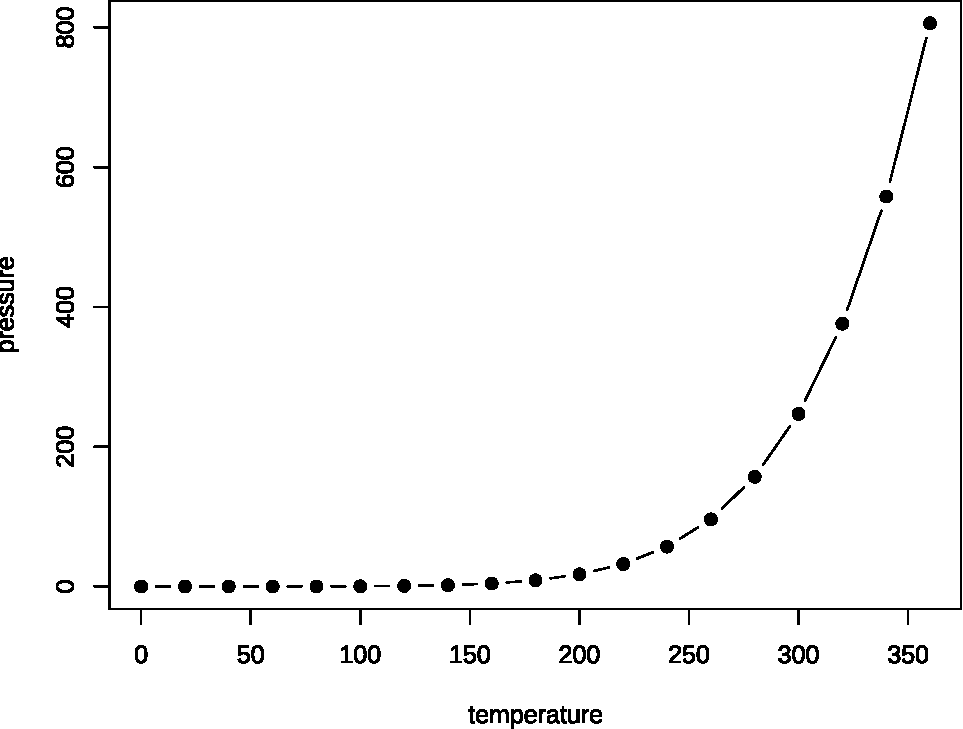
\includegraphics[width=0.8\linewidth]{90-bookdown_files/figure-latex/nice-fig-1} 

}

\caption{Here is a nice figure!}\label{fig:nice-fig}
\end{figure}

Don't miss Table \ref{tab:nice-tab}.

\begin{Shaded}
\begin{Highlighting}[]
\NormalTok{knitr}\SpecialCharTok{::}\FunctionTok{kable}\NormalTok{(}
  \FunctionTok{head}\NormalTok{(pressure, }\DecValTok{10}\NormalTok{), }\AttributeTok{caption =} \StringTok{\textquotesingle{}Here is a nice table!\textquotesingle{}}\NormalTok{,}
  \AttributeTok{booktabs =} \ConstantTok{TRUE}
\NormalTok{)}
\end{Highlighting}
\end{Shaded}

\begin{table}

\caption{\label{tab:nice-tab}Here is a nice table!}
\centering
\begin{tabular}[t]{rr}
\toprule
temperature & pressure\\
\midrule
0 & 0.0002\\
20 & 0.0012\\
40 & 0.0060\\
60 & 0.0300\\
80 & 0.0900\\
\addlinespace
100 & 0.2700\\
120 & 0.7500\\
140 & 1.8500\\
160 & 4.2000\\
180 & 8.8000\\
\bottomrule
\end{tabular}
\end{table}

\hypertarget{parts}{%
\subsection{Parts}\label{parts}}

You can add parts to organize one or more book chapters together. Parts can be inserted at the top of an .Rmd file, before the first-level chapter heading in that same file.

Add a numbered part: \texttt{\#\ (PART)\ Act\ one\ \{-\}} (followed by \texttt{\#\ A\ chapter})

Add an unnumbered part: \texttt{\#\ (PART\textbackslash{}*)\ Act\ one\ \{-\}} (followed by \texttt{\#\ A\ chapter})

Add an appendix as a special kind of un-numbered part: \texttt{\#\ (APPENDIX)\ Other\ stuff\ \{-\}} (followed by \texttt{\#\ A\ chapter}). Chapters in an appendix are prepended with letters instead of numbers.

\hypertarget{footnotes-and-citations}{%
\subsection{Footnotes and citations}\label{footnotes-and-citations}}

\hypertarget{footnotes-1}{%
\subsubsection{Footnotes}\label{footnotes-1}}

Footnotes are put inside the square brackets after a caret \texttt{\^{}{[}{]}}. Like this one \footnote{This is a footnote.}.

\hypertarget{citations-1}{%
\subsubsection{Citations}\label{citations-1}}

Reference items in your bibliography file(s) using \texttt{@key}.

For example, we are using the \textbf{bookdown} package \citep{R-bookdown} (check out the last code chunk in index.Rmd to see how this citation key was added) in this sample book, which was built on top of R Markdown and \textbf{knitr} \citep{xie2015} (this citation was added manually in an external file book.bib).
Note that the \texttt{.bib} files need to be listed in the index.Rmd with the YAML \texttt{bibliography} key.

The \texttt{bs4\_book} theme makes footnotes appear inline when you click on them. In this example book, we added \texttt{csl:\ chicago-fullnote-bibliography.csl} to the \texttt{index.Rmd} YAML, and include the \texttt{.csl} file. To download a new style, we recommend: \url{https://www.zotero.org/styles/}

The RStudio Visual Markdown Editor can also make it easier to insert citations: \url{https://rstudio.github.io/visual-markdown-editing/\#/citations}

\hypertarget{blocks}{%
\subsection{Blocks}\label{blocks}}

\hypertarget{equations-1}{%
\subsubsection{Equations}\label{equations-1}}

Here is an equation.

\begin{equation} 
  f\left(k\right) = \binom{n}{k} p^k\left(1-p\right)^{n-k}
  \label{eq:binom}
\end{equation}

You may refer to using \texttt{\textbackslash{}@ref(eq:binom)}, like see Equation \eqref{eq:binom}.

\hypertarget{theorems-and-proofs-1}{%
\subsubsection{Theorems and proofs}\label{theorems-and-proofs-1}}

Labeled theorems can be referenced in text using \texttt{\textbackslash{}@ref(thm:tri)}, for example, check out this smart theorem \ref{thm:tri}.

\begin{theorem}
\protect\hypertarget{thm:tri}{}\label{thm:tri}For a right triangle, if \(c\) denotes the \emph{length} of the hypotenuse
and \(a\) and \(b\) denote the lengths of the \textbf{other} two sides, we have
\[a^2 + b^2 = c^2\]
\end{theorem}

Read more here \url{https://bookdown.org/yihui/bookdown/markdown-extensions-by-bookdown.html}.

\hypertarget{callout-blocks-1}{%
\subsubsection{Callout blocks}\label{callout-blocks-1}}

The \texttt{bs4\_book} theme also includes special callout blocks, like this \texttt{.rmdnote}.

You can use \textbf{markdown} inside a block.

\begin{Shaded}
\begin{Highlighting}[]
\FunctionTok{head}\NormalTok{(beaver1, }\AttributeTok{n =} \DecValTok{5}\NormalTok{)}
\CommentTok{\#\textgreater{}   day time  temp activ}
\CommentTok{\#\textgreater{} 1 346  840 36.33     0}
\CommentTok{\#\textgreater{} 2 346  850 36.34     0}
\CommentTok{\#\textgreater{} 3 346  900 36.35     0}
\CommentTok{\#\textgreater{} 4 346  910 36.42     0}
\CommentTok{\#\textgreater{} 5 346  920 36.55     0}
\end{Highlighting}
\end{Shaded}

It is up to the user to define the appearance of these blocks for LaTeX output.

You may also use: \texttt{.rmdcaution}, \texttt{.rmdimportant}, \texttt{.rmdtip}, or \texttt{.rmdwarning} as the block name.

The R Markdown Cookbook provides more help on how to use custom blocks to design your own callouts: \url{https://bookdown.org/yihui/rmarkdown-cookbook/custom-blocks.html}

\hypertarget{sharing-your-book}{%
\subsection{Sharing your book}\label{sharing-your-book}}

\hypertarget{publishing-1}{%
\subsubsection{Publishing}\label{publishing-1}}

HTML books can be published online, see: \url{https://bookdown.org/yihui/bookdown/publishing.html}

\hypertarget{pages-1}{%
\subsubsection{404 pages}\label{pages-1}}

By default, users will be directed to a 404 page if they try to access a webpage that cannot be found. If you'd like to customize your 404 page instead of using the default, you may add either a \texttt{\_404.Rmd} or \texttt{\_404.md} file to your project root and use code and/or Markdown syntax.

\hypertarget{metadata-for-sharing-1}{%
\subsubsection{Metadata for sharing}\label{metadata-for-sharing-1}}

Bookdown HTML books will provide HTML metadata for social sharing on platforms like Twitter, Facebook, and LinkedIn, using information you provide in the \texttt{index.Rmd} YAML. To setup, set the \texttt{url} for your book and the path to your \texttt{cover-image} file. Your book's \texttt{title} and \texttt{description} are also used.

This \texttt{bs4\_book} provides enhanced metadata for social sharing, so that each chapter shared will have a unique description, auto-generated based on the content.

Specify your book's source repository on GitHub as the \texttt{repo} in the \texttt{\_output.yml} file, which allows users to view each chapter's source file or suggest an edit. Read more about the features of this output format here:

\url{https://pkgs.rstudio.com/bookdown/reference/bs4_book.html}

Or use:

\begin{Shaded}
\begin{Highlighting}[]
\NormalTok{?bookdown}\SpecialCharTok{::}\NormalTok{bs4\_book}
\end{Highlighting}
\end{Shaded}


  \bibliography{book.bib,packages.bib}

\end{document}
